%!TEX root = ../../../report.tex
\section{3D printing} % (fold)
\label{sec:3d_printing}

  \subsection{Arc compensation} % (fold)
  \label{sub:arc_compensation}
  For the CAD models of the 3D printed parts, the cleareances of the internal holes have been adjusted following \cite{arc_compensation}.
  The undersizing of internal holes is a common problem in this sort of technology due to the lack of information of the common-used exporting format: the STL.
  This only contains the 3D model expressed as a set of external triangles, whichs diffcults the correction of malformations inherent to the technology.

  In the case of the Fused Filament Frabrication (FFF), the material is extrueded equally in both sides of the arc, as shown in \ref{fig:arc_compensation}. 
  However, in the side of the smaller curve, less material is needed.
  This correction can be calculated with:
  $$ r=\frac{t+\sqrt{t^2+4R^2}}{2}$$
  being:
  \begin{enumerate}
    \item t: noozle diameter
    \item R: desired interal hole radius
    \item r: corrected radius
  \end{enumerate}
  As an example, Klee sugests an internal hole of 4.4 mm in the case of the selected nuts \cite{klee}. Thus, the diameter in the CAD model has been adjusted for this data and a noozle of 0.4 mm. The rusult is then:
  $$ d=2r=\frac{t+\sqrt{t^2+4R^2}}{2}=0.4+\sqrt{0.4^2+4*2.2^2}=4.81$$

  \begin{figure}[tb]
    \centering
    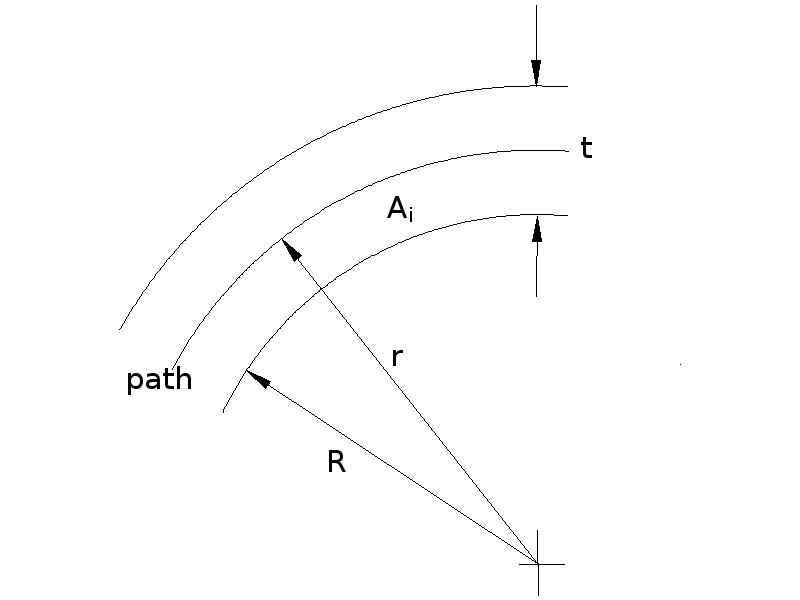
\includegraphics[width=0.5\textwidth]{figures/Arc-compensation}
    \caption{Technical representation of the generated arc when using FFF technology}
    \label{fig:arc_compensation}
  \end{figure}
  % subsection arc_compensation (end)

% section 3d_printing (end)